%TC:group tabular 1 1
%TC:group table 1 1

\chapter{Introduction}

\section{Motivation}

\paragraph{} There exist many programs for music notation and composition. In Sibelius (fig \ref{intro:interfaces} (a)), users write scores using traditional western music notation, whilst music is produced in the live programming interface Sonic Pi (fig \ref{intro:interfaces} (b)) by writing Ruby code~\cite{aaron:pi}. These require users to gain familiarity with a new interface, often with a large threshold to creating simple musical ideas. There are four times more spreadsheet users than programmers~\cite{scaffidi:estimating}, it being the preferred programming language for many people~\cite{blackwell:functions}. I believe that this ubiquituity, along with the affordances of the spreadsheet, would enable new ways to interact with musical notation that capitalise on existing familiarities with spreadsheets and their data handling capabilities.

\paragraph{} The use of grid structures is an established concept in music programs, with most sequencing software using one axis of the screen for time, and the other for pitch or musical parts. Nash's Manhattan~\cite{nash:manhattan} (fig \ref{intro:interfaces} (c)) uses a grid structure where formulae be define a cell's value, like in a spreadsheet. However, it is limited to columns defining tracks and rows corresponding to time. Sarkar's SheetMusic~\cite{sarkar:sheetmusic} investigated including formulae with sound output within the spreadsheet paradigm. This also introduced abstracting time away from the grid, in this case using an incrementing global \texttt{tick} variable which could be referred to in formulae. Both axes can be used interchangeably for SheetMusic notation or non-musically interpreted markup that the user wishes to include, a concept idiomatic to Excel usage. Simple formulae such as \texttt{if(tick\%2==0) p('snare') else p('kick')} allow musical structures to be defined without advanced programming knowledge but quickly become unwieldy for larger pieces, especially if they are not highly repetitive. Whilst other spreadsheet music projects exist~\cite{hackaday:spreadsheet}, these simply use the spreadsheet as the medium for conventional sequencing with an auxiliary script to parse the grid and create musical output.

\paragraph{} Excello (fig \ref{intro:interfaces} (d)) is an Excel add-in for end-user music programming where users define music in the spreadsheet and can play it back from within Excel. It maintains the abstraction of time from the grid to keep the flexibility spreadsheets offer, but was designed so individual cells would not become too complex. Existing Excel functionality can be used, both accelerating the learning curve and increasing the available functionality.

\begin{figure}[ht]
\begin{tabular}{cc}
  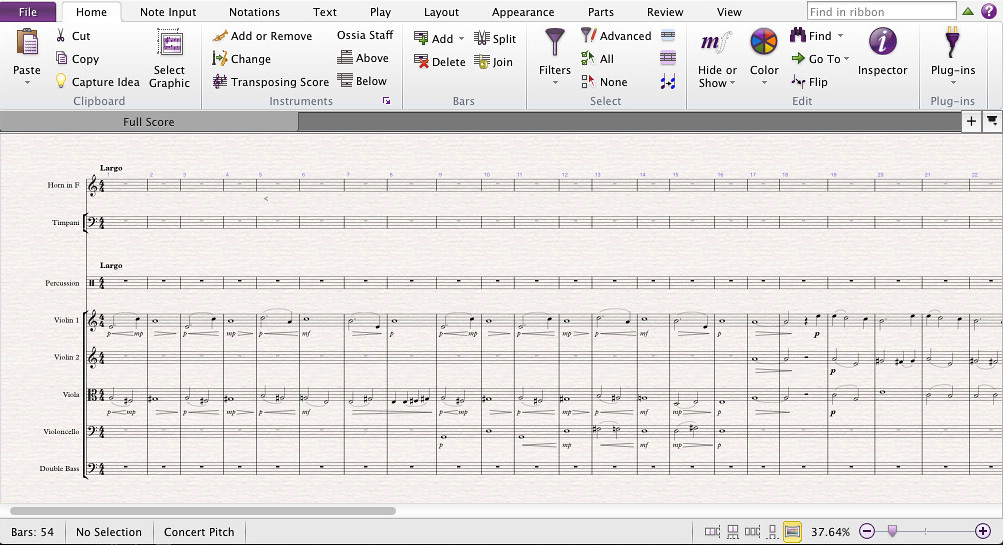
\includegraphics[width=75mm]{figs/sib.jpg} & 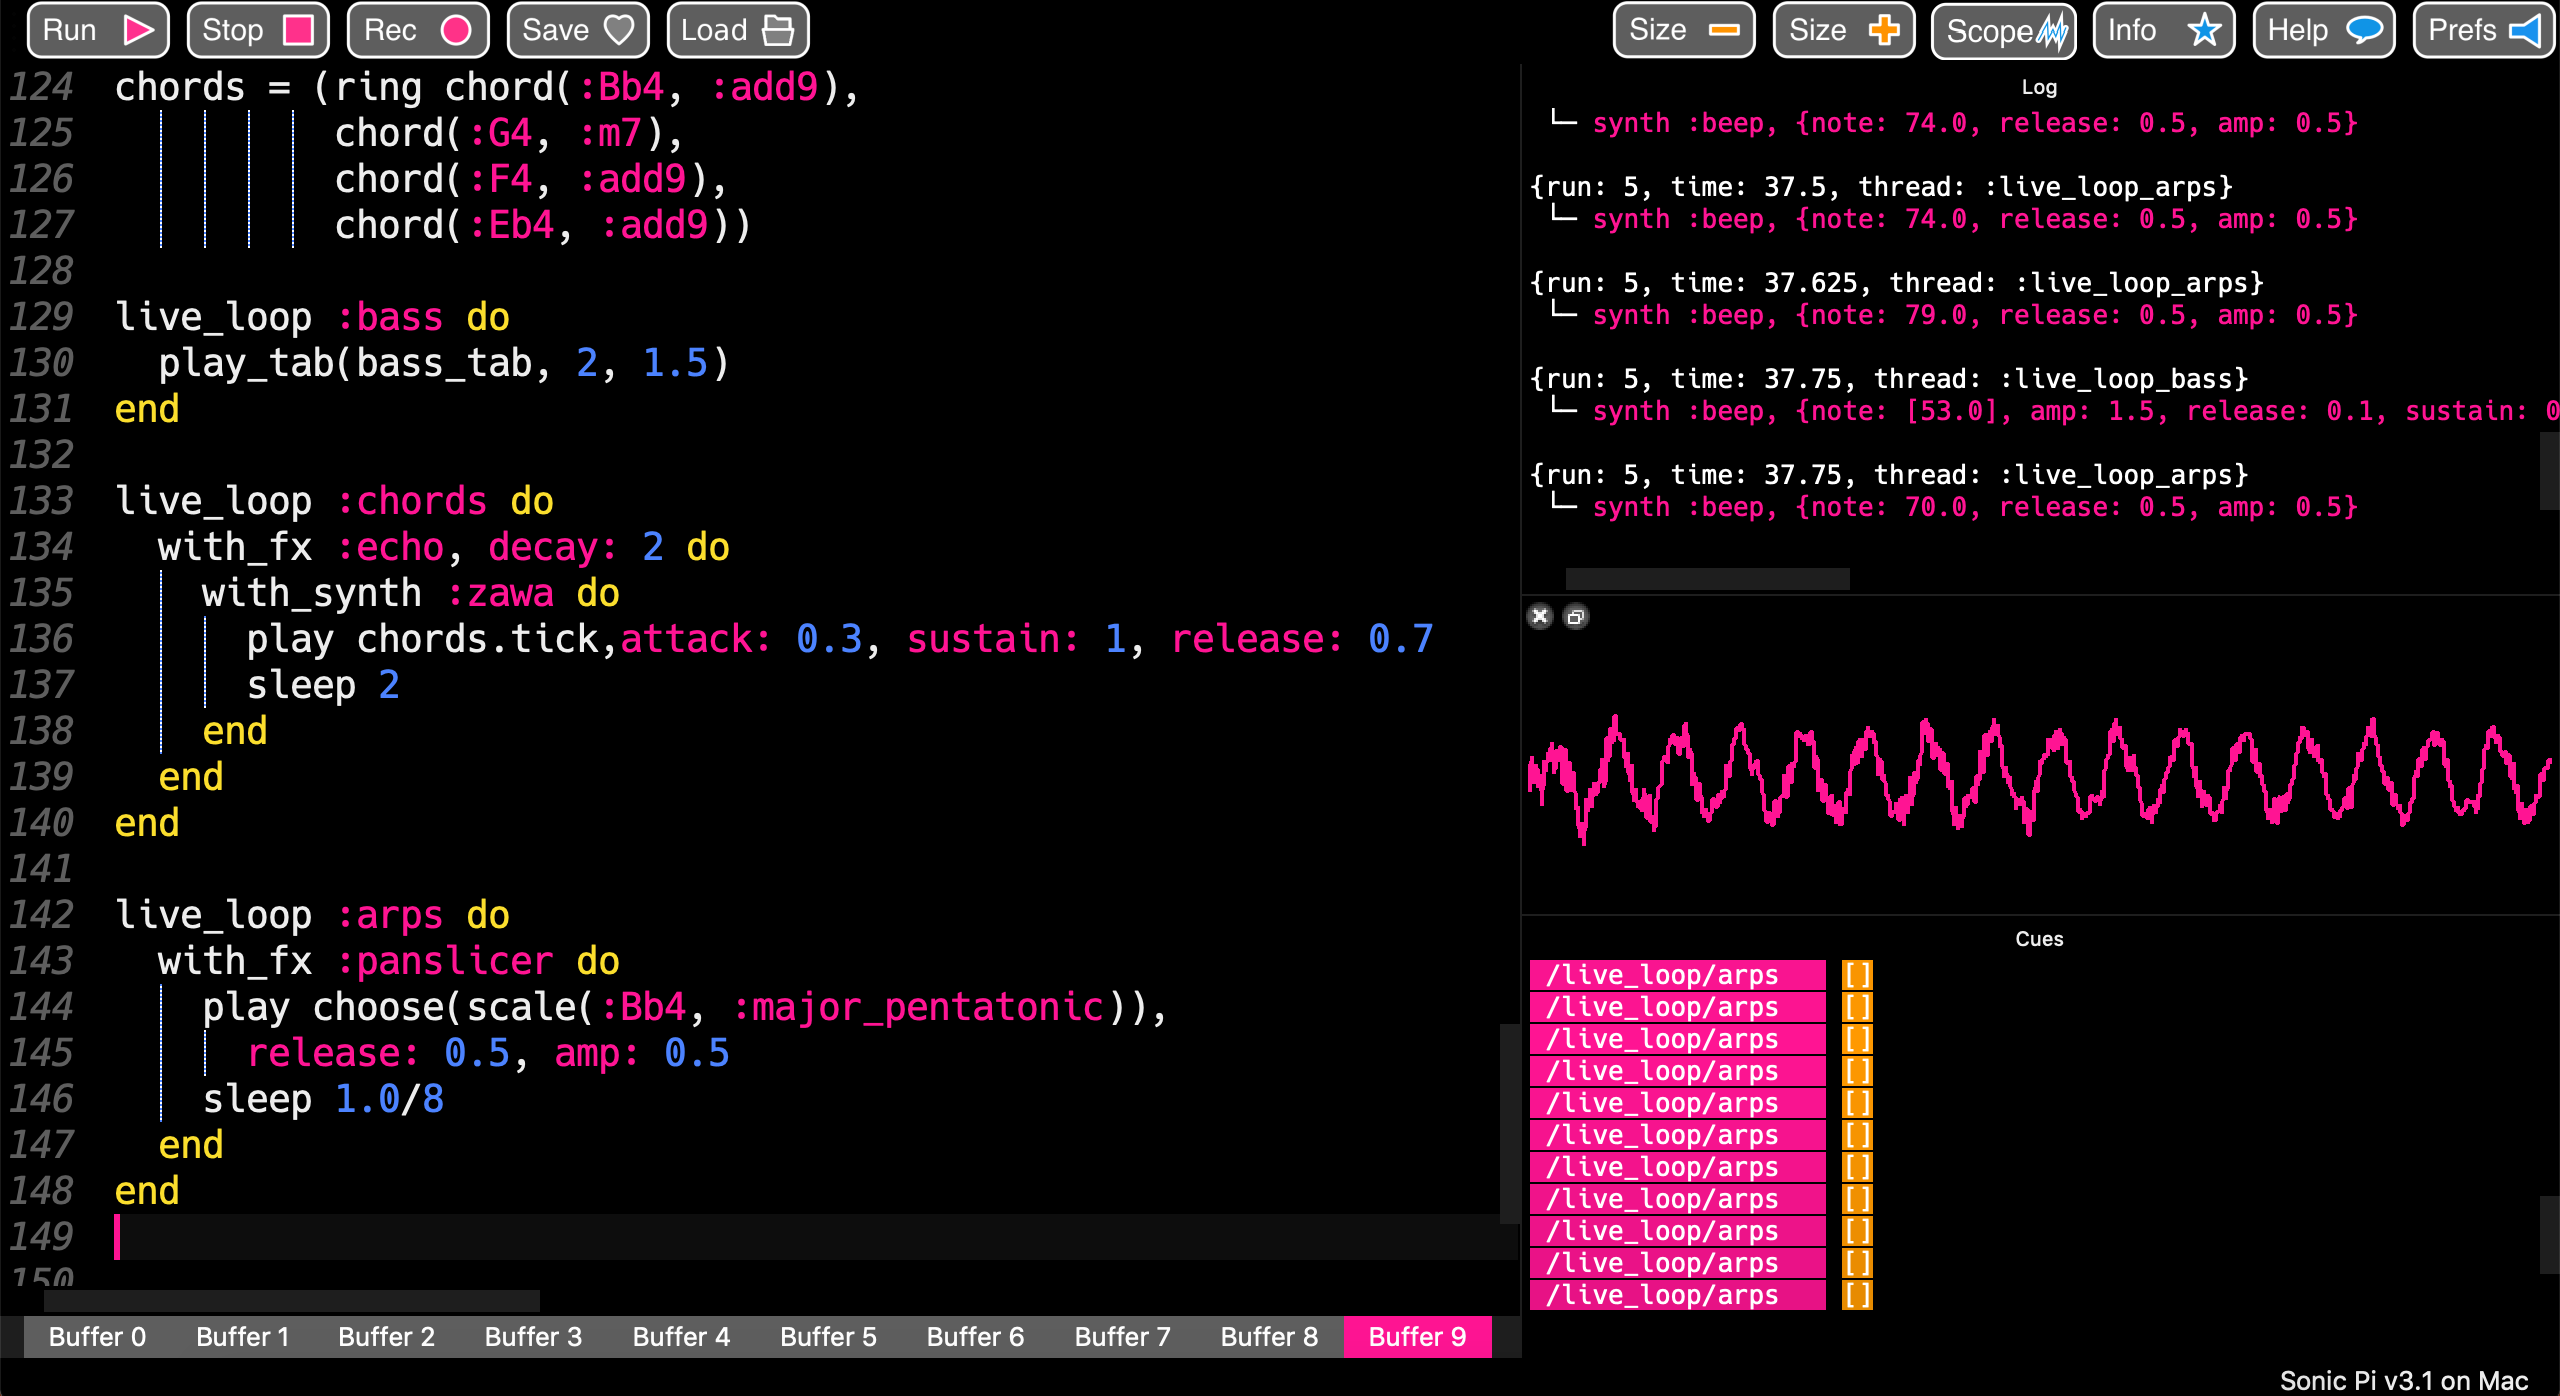
\includegraphics[width=75mm]{figs/sonicPi.png} \\
  (a) Sibelius - an editor with playback for&(b) Sonic Pi - code is written on the left\\
  staff notation \textcopyright\ Gorazd Bozic\footnote{https://creativecommons.org/licenses/by-nc/2.0/.}& and output information on the right \\
  & \\
  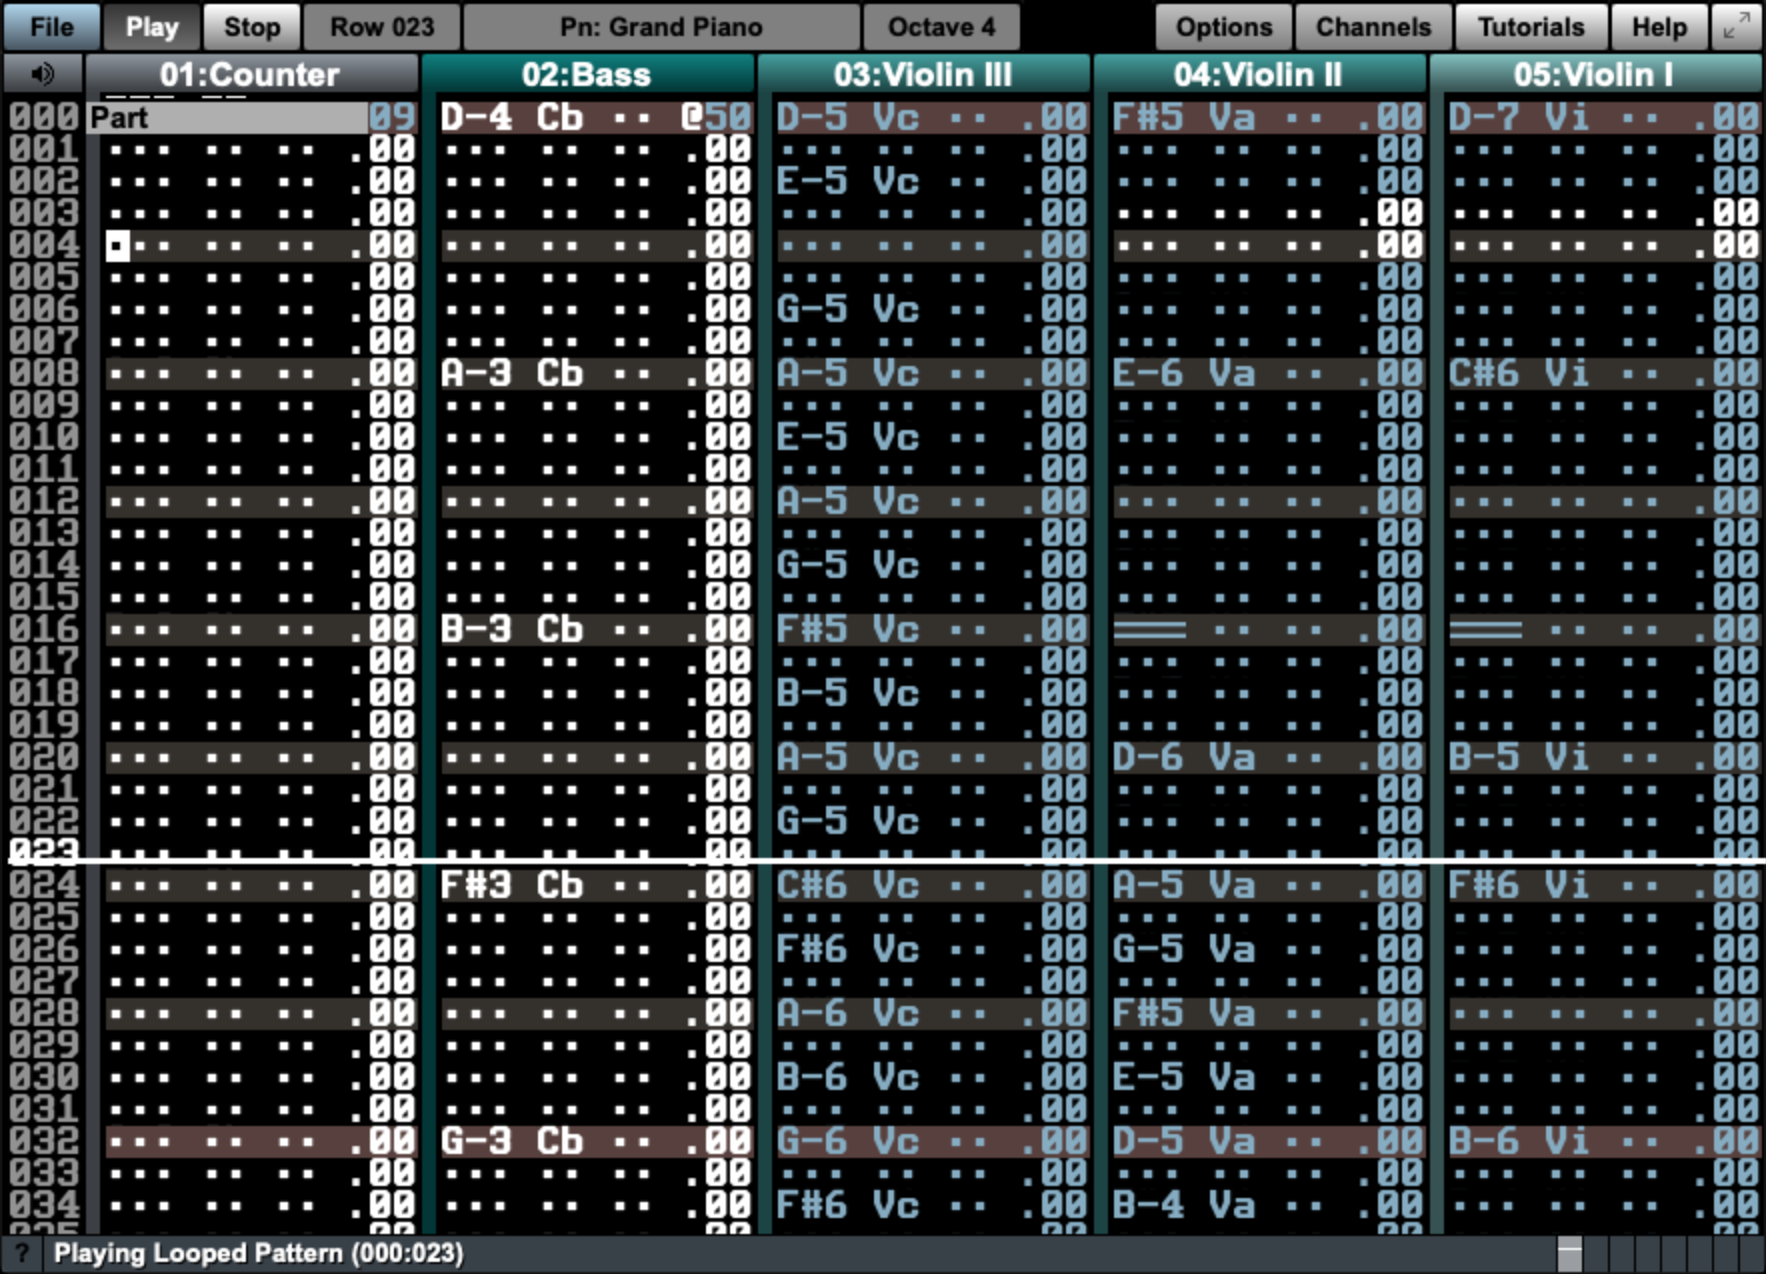
\includegraphics[width=75mm]{figs/manhattan.png} & 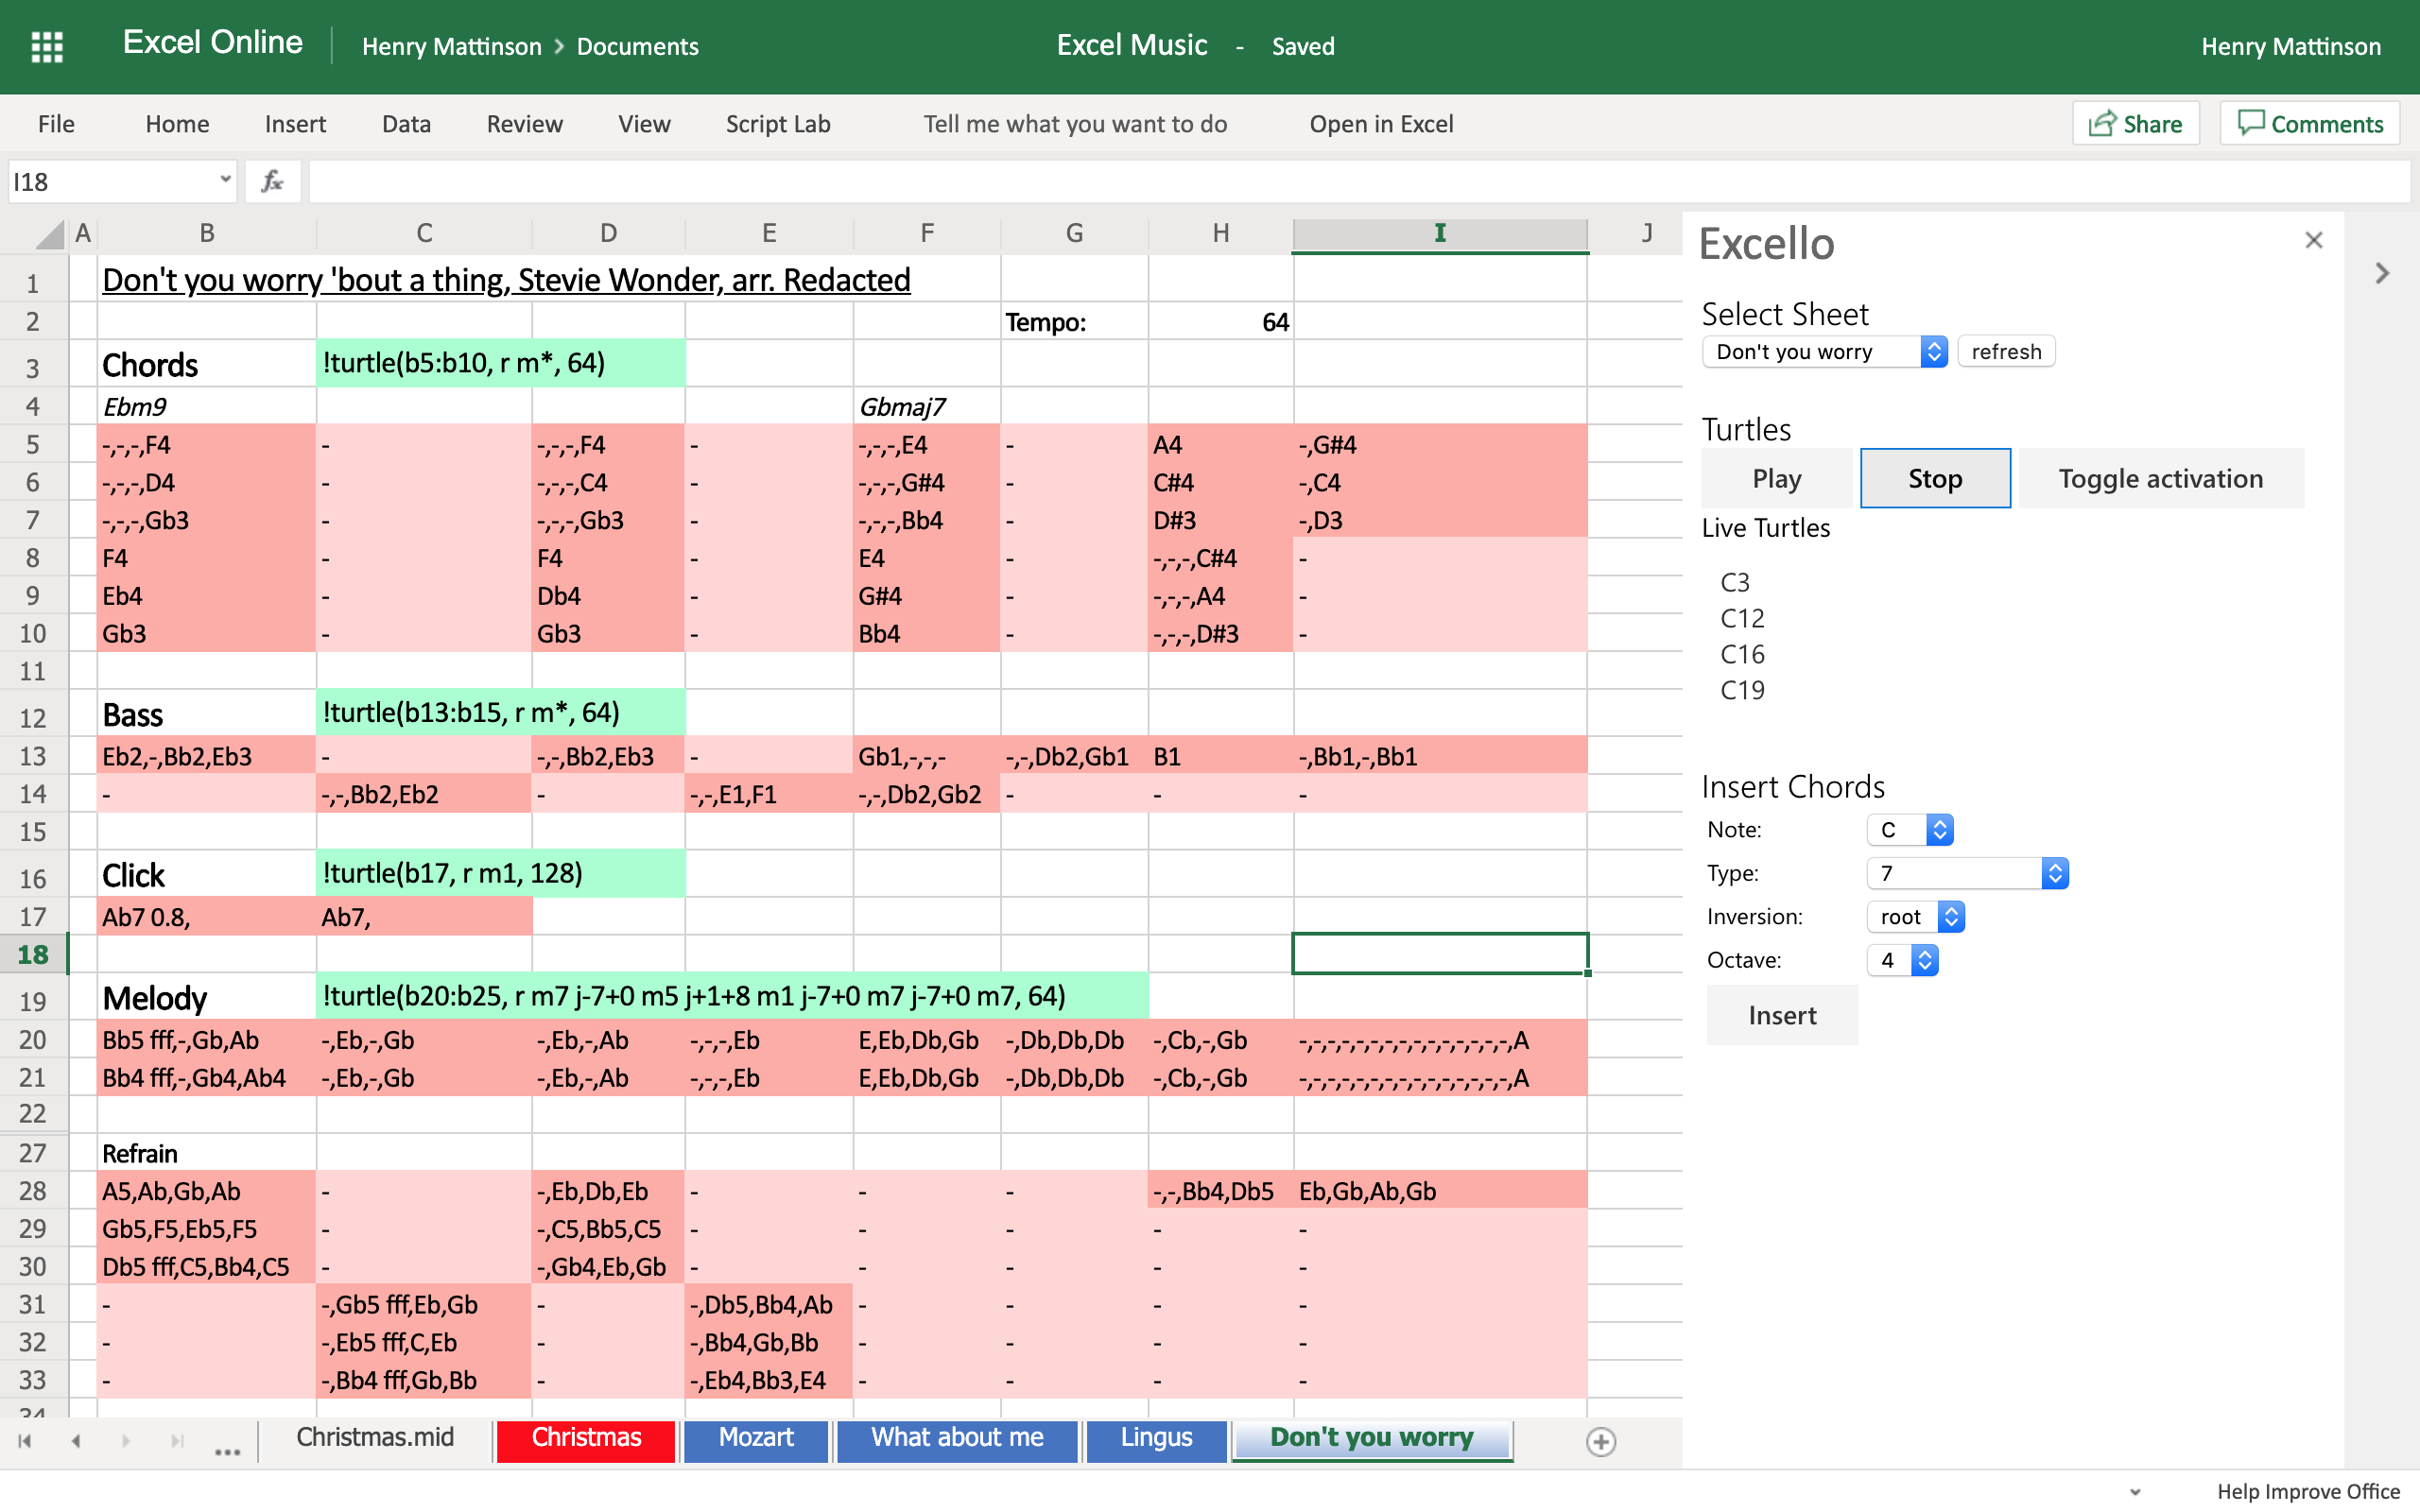
\includegraphics[width=75mm]{figs/excelloFull.png} \\
  (c) Manhattan - columns of parts played&(d) Excello - a spreadsheet of music notation\\
  from top to bottom&with a window for playback on the right\\
\end{tabular}
\caption{The interfaces of (a) Sibelius, (b) Sonic Pi, (c) Manhattan, (d) Excello}
\label{intro:interfaces}
\end{figure}

\vspace{-10pt}

\section{Outline of work}

\begin{enumerate}

\item I designed and built a prototype for musical expression and playback within Excel satisfying the all the success criteria for the system.

\item Participatory design began using this initial prototype. Following formative evaluation sessions with 21 participants, issues and feature requests were identified. Users continued to give feedback as they used the updated prototypes.

\item A series of extensions were implemented, solving problems identified by participants and adding requested features.

\item A converter from MIDI to the Excello format was built and a large MIDI corpus translated.

\item Summative evaluation was performed with the participants. Evaluating the features implemented during participatory design and Excello's usability using the Cognitive Dimensions of Notation (CDN) framework~\cite{blackwell:tutorial}, using Sibelius as a comparison.

\end{enumerate}
